\documentclass[11pt]{scrartcl}
\usepackage[top=1cm, bottom=2.5cm, left=2.5cm, right=2.5cm]{geometry}
\usepackage{graphicx,float,enumerate}
\usepackage{url}
\usepackage[T1]{fontenc}
\usepackage[font=small,labelfont=bf,tableposition=top]{caption}
\usepackage{amsmath,amssymb,amsfonts}
%\usepackage{algorithm, algorithmic}
%opening
\usepackage{titling}
\usepackage{multirow}
\setlength{\droptitle}{-2cm}
\title{Project Report 3}
\author{Fuyuan Lyu, Tianyu Shi, Dingyi Zhuang}

\begin{document}

\maketitle

\begin{abstract}
In this project, we build several models to classify image data. We use the CIFAR 10 dataset with the default test and train partitions.
Then we build several models, including Multilayer perceptron, Convolutional Neural Network. We have done several experiments on preprocessing methods, neural network structure, and parameter tuning.
\end{abstract}
  
\section{Introduction}
The goal of this project is to investigate the performance of different models upon the CIFAR-10 dataset. The CIFAR-10 dataset is a collection of images that are commonly used to train machine learning and computer vision algorithms. The CIFAR-10 dataset contains 60,000 32x32 color images in 10 different classes.The 10 different classes represent airplanes, cars, birds, cats, deer, dogs, frogs, horses, ships, and trucks. There are 6,000 images of each class.

In the pre-processing stage, we have tried several data augmentation techniques, including Using the Random Horizontal Flip, Random Crop Transforms and Normalization on both training and testing sets. Data augmentation can make our trained models more robust and capable of achieving higher accuracy without requiring a larger dataset.
We have also tried to normalize the image dataset. All values in the image data set originally ranges from 0 to 255. When the back-propagation process is performed to optimize the networks, this could lead to an exploding/vanishing gradient problems. To avoid the issue, it is better to let all the values be around 0 and 1.
Furthermore, we also tried one-hot encoding for each label. A vector having the same number of elements as the number of classes of the image is implemented. For instance, CIFAR-10 provides 10 different classes of the image, so we build a vector in size of 10 as well, which can guarantee our models to do a better job in the prediction period.



\section{Related Work}
The Image classification task is a classical problem in the computer vision field. In this task, models take the pixel-based images as input and aim to successfully classify it to given labels. When multilayer perceptron is processing such tasks, it vectorizes the whole images and ignores the spatial structure of the image. One multilayer perceptron has the characteristic of fully connected layers and consists of at least three such layers. The pro is that all neurons have the feedforward information of all neurons from the previous layer, while the con is that this mechanism may contain too many weights and prone to overfitting.

Later, multilayer perceptron is deemed insufficient for more advanced computer vision tasks and replaced by convolutional neural network\cite{krizhevsky2012imagenet}, which uses convolution operation as the basic component, after its success in ImageNet challenge\cite{deng2009imagenet}. Nowadays, the structure of convolutional neural network has evolved and changed a lot from the original structure. But in this project, we will stick the classic version.



\section{Dataset preprocessing}
We use the CIFAR-10 dataset to train and test our model. The original one batch data is (10000 x 3072) matrix expressed in NumPy array. The number of columns, (10000), indicates the number of sample data. As stated in the CIFAR-10 dataset, the row vector, (3072) represents a color image of 32x32 pixels. 
We reshape and transpose the original input image data in the form of $width \times height \times num_{channel}$ in order to feed it into our models.
We then build the normalization function which takes data, x, and returns it as a normalized Numpy array. In our model, x is a  3-D array for an image. Min-Max Normalization (y = (x-min) / (max-min)) technique is used to transform the original image into the range of 0 to 1. 
Furthermore, we build one hot encode function which takes the input, x, which is a list of labels(ground truth). The total number of elements in the list is the total number of samples in a batch. One hot encode function returns a 2-dimensional tensor, where the number of rows is the size of the batch, and the number of columns is the number of image classes.
Finally, we apply several data augmentation techniques for both training and testing parts. A typical example of augmented image sets is shown in figure \ref{data_aug}.

\begin{figure}[H]
	\centering
	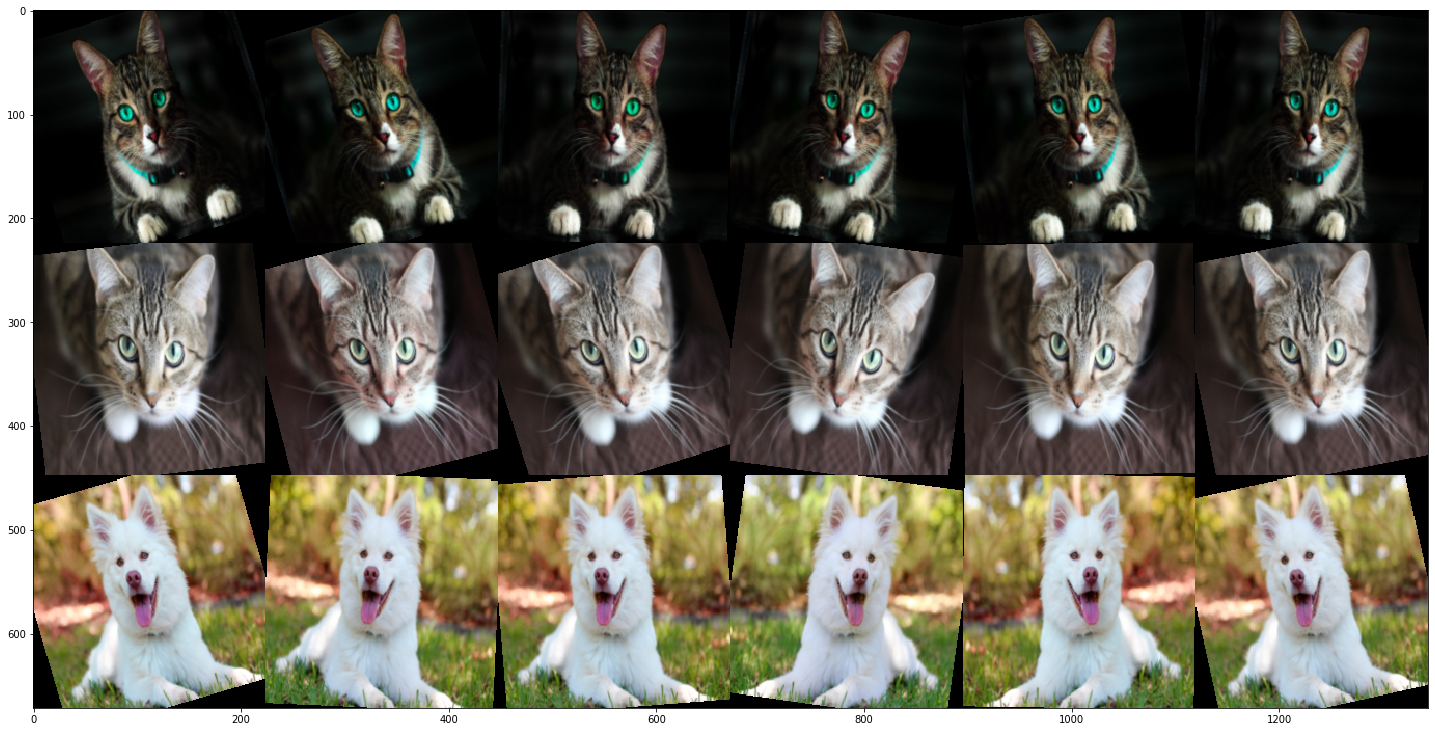
\includegraphics[width=0.9\linewidth]{fig/random_flip_crop_padding.png}
	\caption{Data augmentaion technique based on random flip and crop}
	\label{data_aug}
\end{figure}

\section{Proposed approach}
Our approaches consist of two parts: multilayer perceptron and convolutional neural network.
\subsection{Multilayer perceptron}
We implement multilayer perceptron from scratch. We find that the most difficult parts lie in
\begin{enumerate}[(1)]
	\item How to construct the whole structure of multilayer perceptron
	\item How to backpropagate the errors
	\item How to optimize the backpropagation to make it not oscillate around the initial values
\end{enumerate}
We will introduce the building mechanism for our work by answering these three questions.

Firstly, in order to give a clear representation of the layer, we define a parent class layer as a programming object, which contains the summation vector of $wz+b$, the activation function, loss difference, and gradient deviation, etc. You can check the code in \texttt{layer.py}. The activation function we use here is ReLU instead of sigmoid because it is more widely applied. Inherited from basic layer parent class, we define three major layers: \textit{input\_layer}, \textit{hidden\_layer} and \textit{output\_layer}. \textit{input\_layer} and \textit{output\_layer} have a slight difference from their parent class, the former does not accept any output and is a container for the input data. As for the output layer, we connect it with the last hidden layer and choose \textit{softmax} as its output results. So you can find that the output layer has its special attribute \textit{output\_layer.output}. The advantage of defining such class of layers is that we can stack multiple layers when we build the multilayer perceptron, instead of directly defining the weights and bias matrices as many blogs do. You can check-in in \textit{MLP.build\_net} in \texttt{mlp.py}.

Secondly, we think the most difficult part of implementing the multilayer perceptron is the backpropagation. Let's look at the \textit{MLP.train\_fit}, we flatten the input three-channel figure into a one-dimensional vector. After we feed-forward the network to calculate the activations, we first compute the backpropagation error. By implementing a similar code from the slides, we use the one-hot encoding target minus the softmax probability as the output error. And then, we backpropagate this error by multiplying weights and derivative of activation functions. If we consider the backpropagation procedure in the slides as
\begin{equation*}
	\frac{\partial}{\partial V_{m,d}} = \sum_{c} \frac{\partial L}{\partial \hat{y}_c} \frac{\partial \hat{y}_c}{\partial u_m} \frac{\partial u_m}{\partial z_m} \frac{\partial z_m}{\partial q_m} \frac{\partial q_m}{\partial V_{m,d}}
\end{equation*}
Then \textit{MLP.back\_propgation\_error} computes the 

$$\sum_{c} \frac{\partial L}{\partial \hat{y}_c} \frac{\partial \hat{y}_c}{\partial u_m} \frac{\partial u_m}{\partial z_m} \frac{\partial z_m}{\partial q_m}$$

And then we add \textit{MLP.compute\_gradients\_errors} to make it complete. 

But the backpropagation is not yet stable, we, therefore, add stochastic gradient descent (SGD) with momentum to make the optimization stable in \textit{MLP.compute\_gradients\_errors}. We are confused for a very long time about our accuracy as it is only 0.1 in the beginning, which is only the oscillation around the initialization values. We then realize that it is because of the unstable property of SGD. So we add the momentum term for more stable learning with $\beta = 0.9$:

\begin{align*}
	\Delta w^{\{t\}} & \gets \beta \Delta w^{\{t-1\}} + (1-\beta) \nabla J (w^{\{t\}})\\
	w^{\{t\}} & \gets w^{\{t-1\}} - \alpha \Delta w^{\{t\}}
\end{align*}

After the update the gradient updates, it would be very easy to implement the rest of the part.

\subsection{Convolutional neural network}
Our implementation of Convolutional neural network is based on the PyTorch documentation example, but we
\begin{enumerate}[(1)]
	\item Use \textit{nn.ModuleList} to make adding any numbers of convolutional layers and fully connected layers possible.
	\item Add comments on each reused code line. 
\end{enumerate}
Because it is reused from the documentation and commented, there are no more details to emphasize.

\section{Results}
In the experiment stage, we will compare the performance of multilayer perceptron and convolution neural network on CIFAR10 dataset\cite{krizhevsky2009learning}. We also perform hyper-parameter tuning for both models.


\subsection{Hyper-parameter tuning for multilayer perceptron}
When tuning hyper-parameters for multilayer perceptron, we try different learning ratios, activation functions, and training epochs. We also compare our implemented-from-scratch version multilayer perceptron with an implementation based on PyTorch, as shown in Table \ref{MLP}.


\begin{table}[H]
	\centering
	\begin{tabular}{c|cccccc}
		\hline
		  config. & units & source & epochs & activation function & learning ratio & accuracy  \\
		\hline
		  a & (120, 84) & - & 10 & ReLU & 1e-3 & 0.2715 \\
		 \hline
		  b & (120, 84) & - & 30 & ReLU & 1e-3 & 0.2804 \\
		  c & (120, 84) & - & 3  & ReLU & 1e-3 & 0.2691 \\
		 \hline
		  d & (120, 84) & - & 10 & ReLU & 1e-4 & 0.2642 \\
		  e & (120, 84) & - & 10 & ReLU & 1e-2 & 0.2829 \\
		 \hline
		  f & (360,140) & - & 10 & ReLU & 1e-3 & 0.3125 \\
		  g & (180,120) & - & 10 & ReLU & 1e-3 & 0.3038 \\
		  h & (60, 40)  & - & 10 & ReLU & 1e-3 & 0.2478 \\
		 \hline
		  i & (120, 84) & - & 10 & Sigmoid & 1e-3 & 0.2198 \\
		  j & (120, 84) & - & 3  & Sigmoid & 1e-3 & 0.2086 \\
		 \hline
		  k & (120, 84) & pytorch & 10 & ReLU & 1e-3 & 0.521 \\
		  l & (120, 84) & pytorch & 3  & ReLU & 1e-3 & 0.491 \\
		\hline
	\end{tabular} 
	\caption{Hyper-parameter tuning for multilayer perceptron}
	\label{MLP}
\end{table}

Here we treat configuration a as default configuration and conduct control variable experiment based on that. Configuration b and c investigate the influence of the training epoch. The increase in the training epoch does lead to an increase in the final performance. Configuration d and e try to tune the learning ratio. It is shown that a higher learning ratio may lead to a better model performance given the current design. Configuration f, g, and h investigate the influence of the number of neurons for each hidden layer. Multilayer perceptrons with more hidden neurons are prone to capture more features and lead to an accurate result. Configuration i and j try to switch the activation function after each fully connected layers. The sigmoid function does not perform as good as the ReLU function. Configuration k and l compare our implementation with PyTorch implementation of multilayer perceptron.

\subsection{Hyper-parameter tuning for convolutional neural network}

When tuning hyper-parameter for convolutional neural networks, we try different optimizers, layer numbers, channels, and activation functions. Here we set the learning ratio to be 1e-3 and the activation function as ReLU. The structure of the classifier is the same as the default structure for the previous multilayer perceptron, which is an MLP with 2 hidden layers and 120, 84 neurons for each layer correspondingly. The training epoch is set to 10 as default. The result is shown in Table \ref{CNN}.

\begin{table}[H]
	\centering
	\begin{tabular}{c|cccc}
		\hline
		config. & layer nums & channel numbers & Optimizer & accuracy  \\
		\hline
		a & 2 & (6, 16) 	& SGD  & 0.639 \\
		b & 2 & (24, 36) 	& SGD  & 0.680 \\
		c & 2 & (6, 16)  	& Adam & 0.644 \\
		d & 2 & (24, 36) 	& Adam & 0.661 \\
		e & 3 & (6, 16, 16) & SGD  & 0.616 \\
		f & 3 & (24,36, 36) & SGD  & 0.705 \\
		\hline
	\end{tabular} 
	\caption{Hyper-parameter tuning for convolutional neural network}
	\label{CNN}
\end{table}

As we can see from Table \ref{CNN}, configuration a and b different from each other via channel number and the increase of channel number does lead to an increase of accuracy on the test dataset. By comparing configuration c, d with configuration a and b, it can be seen that Adam does not necessarily surpass predecessor optimizers like SGD, which is also proven by other researchers\cite{reddi2019convergencee}. Configuration e and f also prove that simply increasing the depth of the neural network does not necessarily leads to the increase of the model performance. Instead, more delegate design is required. 


\section{Statement for Contributions}


\begin{itemize}
	\item Fuyuan Lyu: Experiment evaluation and writing report
	\item Tianyu Shi: Image pre-processing and writing report
	\item Dingyi Zhuang: Implementation of models and writing report
\end{itemize}
% \newpage

\bibliographystyle{unsrt}
\bibliography{ref}

\end{document}
